\documentclass{ltxdoc}

\usepackage[bookmarks,colorlinks,pdfauthor={Henrik Tidefelt},pdftitle={blockdraw_mp}]{hyperref}
\usepackage[american]{babel}
\usepackage{lmodern}
\usepackage[T1]{fontenc}
\usepackage[latin1]{inputenc}
\usepackage{graphicx}
\usepackage{tiddetext}
\usepackage[squaren]{SIunits}
\usepackage[labelsep=period,font={small,sl}]{caption}
\usepackage[2ex]{tighttoc} % must be loaded before parskip!
\usepackage{parskip}
\usepackage[addtotoc]{abstract}

\title{The \emph{blockdraw\_{}mp} package\\
{\large MetaPost macros for the creation of block diagrams and bond graphs}}
\author{Henrik Tidefelt\\
{\small tidefelt@isy.liu.se}}

\begin{document}
\maketitle

\begin{abstract}
This is not the right place to motivate why MetaPost should be used for the production of technical illustrations, in particular those to be used in material produced using \LaTeX{}.  Block diagrams are no exception since consistent layout of blocks, arrangement of connections, formatting of labels, placement of labels, et~c{} are such demanding tasks.  This package provides macros that facilitate the drawing of block diagrams using MetaPost.  To extend the capabilities to bond graphs is a small step, and such macros are also included in this package.

This document describes the package, but is not the main manual.  However, the $2$-sided appendix starting on an odd page may be used on its own as a reference sheet.
\end{abstract}

\tableofcontents

\newpage

\section{Motivation}%
%
The pdf format has several advantages to PostScript, perhaps most importantly that previewers for pdf are more generally available and of better quality. This is obviously the reason why there is pdf(La)\TeX{}.  However, one problem for some potential pdf(La)\TeX{} users is that the psfrag package is not compatible with pdf(La)\TeX{}.  On the other hand, since psfrag is not the most convenient way of putting good looking labels in a figure anyway, alternatives should be welcome.  The drawing-language MetaPost is a powerful option for those who do not fear the expressiveness of text-based computer languages.  This packages provide macros that facilitate the drawing of block diagrams and bond graphs in MetaPost.  Two examples are given in \figuresref{demo1} and~\fgref{demo2}.

Also the user who have no experience of MetaPost but needs a way to draw nice block diagrams without too much effort should consider using this package, because it might well be worthwhile to learn the few necessary bits of MetaPost.  This typically amounts to looking at a few examples, learning how to invoke the MetaPost interpreter, and get acquainted with the \emph{MetaPost output} format.

\begin{figure}[tbp]
  \fglabel{demo1}
  \centering
  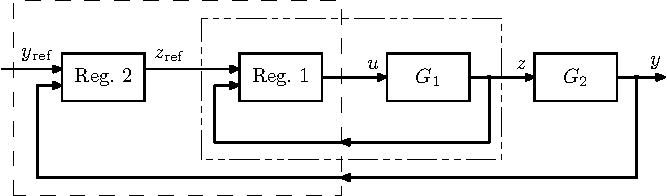
\includegraphics{cascadedemo}
  \caption{Example figure: block diagram.}
\end{figure}

\begin{figure}[tbp]
  \fglabel{demo2}
  \centering
  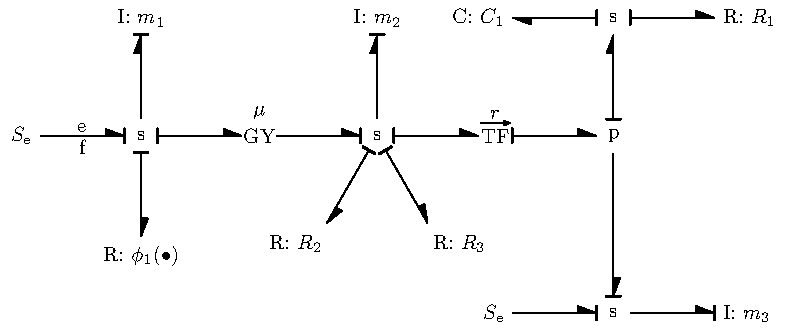
\includegraphics{bonddemo}  
  \caption{Example figure: bond graph.}
\end{figure}


\section{The Full Name}%
%
Although the main implementation file of this package is called \emph{blockdraw.mp}, the package has not been given the name \emph{blockdraw}.  The full name of the package is precisely \emph{blockdraw\_{}mp}, and the reason for this is that the idea of drawing block diagrams with abstractions like those of this package can easily be, have been, and will be implemented in other languages than the presently targeted language MetaPost.  For example, the implementation\footnote{%
Note that it is not a well defined language that is implemented, but merely an idea of how to organize the drawing of block diagrams.
} % The preceding whitespace matters to LaTeX!
I have been using mostly myself was for the language Drool (written by the author, not yet published).  Nevertheless, the present implementation have been used successfully by several others, and support have been provided whenever asked for.  Hence, although I am not a user of the package myself, I am convinced that it is truly useful.

\section{This Document and the WWW-Based Documentation}%
%
The documentation provided in the appendix is meant to be only a brief summary of the variables and macros defined by the MetaPost-hosted package for drawing block diagrams and bond graphs.  Details, illustrations, and examples can be found in the WWW-based documentation, currently available at \href{http://www.control.isy.liu.se/~tidefelt/projects/blockdraw/}{http://www.control.isy.liu.se/$\sim$tidefelt/projects/blockdraw/}.  Still, the appendix might be useful as a reference sheet.

\section{Files}%
%
The implementation consists of three files, which are located in the \emph{implementation} directory:
\begin{itemize}
\item \emph{shiftoff.mp} contains general-purpose macros for placing objects relative to a point.  This file is included from \emph{blockdraw.mp}.
\item \emph{blockdraw.mp} contains the things that are specific to drawing block diagrams.
\item \emph{bondgraph.mp} contains additional macros that are useful when drawing bond graphs.
\end{itemize}

The documentation and the sources needed to compile it are located in the \emph{documentation} directory:
\begin{itemize}
\item \emph{blockdraw\_mp.tex} is the source of this document.
\item \emph{blockdraw\_mp.pdf}
\item \emph{tiddetext.sty} contains various macros used.
\item \emph{tighttoc.sty} is my ugly solution to make the table of contents consume less vertical space.  Perhaps someone would like to have a look at it and make it a proper package\ldots
\item \emph{cascadedemo.mp} is the source of the first demo figure.
\item \emph{cascadedemo.pdf}
\item \emph{bonddemo.mp} is the source of the second demo figure.
\item \emph{bonddemo.pdf}
\item \emph{docblockprefs.mp} is a file with settings to be used in block diagrams produces for this document.  (Currently, there is only one such figure.  A similar file could be creaded for bond diagrams to further emphasize how settings should be factored out in separate files, but I didn't just for brevity.)
\end{itemize}

% Make sure that the appendix starts at an odd page, so that it can be printed selectively.
\newpage
~\\
\newpage

\appendix

\scriptsize

\section{Miscellaneous macros}

\begin{center}
  \begin{tabular}{l c p{5cm}}
    \hline
    \textbf{Name} & \textbf{Argument list} & \textbf{Description} \\
    \hline
    \hline
    \funname{mspoint} & ( \varname{con}, \varname{mediation}, \varname{slide} ) & Alternative to \texttt{point\ldots of\ldots}. \\
    \funname{to\_{}dir} & ( \varname{pt} ) & (Low-level) Converts a direction vector to a direction constant. \\
    \funname{dir\_{}to} & ( \varname{dir} ) & (Low-level) Converts a direction constant to a direction unit vector. \\
    \funname{shiftoff} & ( \varname{pic}, \varname{corner} ) & Places \varname{pic} relative to the origin, according to \varname{corner} which shall be a direction constant (see below). \\
    \funname{shiftoffwlm} & ( \varname{pic}, \varname{corner} ) & Like \funname{shiftoff}, but with ``label margin''. \\
    \hline
  \end{tabular}
\end{center}

\section{Block macros}

\begin{center}
  \begin{tabular}{l c p{5cm}}
    \hline
    \textbf{Name} & \textbf{Argument list} & \textbf{Description} \\
    \hline
    \hline
    \funname{sizedblock} & ( \varname{pict}, \varname{center}, \varname{rx}, \varname{ry} ) & For subsystems of explicitly specified size. \\
    \funname{longblock} & ( \varname{pict}, \varname{center} ) & For subsystems. \\
    \funname{squareblock} & ( \varname{pict}, \varname{center} ) & For simple subsystems. \\
    \funname{roundblock} & ( \varname{pict}, \varname{center} ) & For, for example, summations. \\
    \funname{splitdot} & ( \varname{center} ) & A split point, drawn as a dot. \\
    \funname{termcircle} & ( \varname{center} ) & A connection/terminal point, drawn as a small circle. \\
    \funname{pointpicture} & ( \varname{center} ) & A <typename>picture</typename> that only serves to define a coordinate pair. \\
    \funname{conlabel} & ( \varname{shiftdir}, \varname{pict}, \varname{z} ) & Similar to \funname{label}, but honors the \varname{textscale} setting. \\
  \end{tabular}
\end{center}

\section{Point macros}

\begin{center}
  \begin{tabular}{l c p{5cm}}
    \hline
    \textbf{Name} & \textbf{Argument list} & \textbf{Description} \\
    \hline
    \hline
    \funname{leftpoint} & ( \varname{pict}, \varname{total}, \varname{index} ) & For connections on the left side. \\
    \funname{rightpoint} & ( \varname{pict}, \varname{total}, \varname{index} ) & For connections on the right side. \\
    \funname{bottompoint} & ( \varname{pict}, \varname{total}, \varname{index} ) & For connections on the bottom side. \\
    \funname{toppoint} & ( \varname{pict}, \varname{total}, \varname{index} ) & For connections on the top side. \\
  \end{tabular}
\end{center}

\section{Connection macros}

\begin{center}
  \begin{tabular}{l c p{5cm}}
    \hline
    \textbf{Name} & \textbf{Argument list} & \textbf{Description} \\
    \hline
    \hline
  \funname{hhconnect} & ( \varname{point1}, \varname{point2}, \varname{mediation}, \varname{slide} ) & For horizontal to horizontal connections. \\
  \funname{vvconnect} & ( \varname{point1}, \varname{point2}, \varname{mediation}, \varname{slide} ) & For vertical to vertical connections. \\
  \funname{hvconnect} & ( \varname{point1}, \varname{point2} ) & For horizontal to vertical connections. \\
  \funname{vhconnect} & ( \varname{point1}, \varname{point2} ) & For vertical to horizontal connections. \\
  \funname{connect} & ( \varname{pict1}, \varname{pict2} ) & Automatic side to automatic side. \\
  \funname{lrconnect} & ( \varname{pict1}, \varname{pict2} ) & Left side to right side. \\
  \funname{rlconnect} & ( \varname{pict1}, \varname{pict2} ) & Right side to left side. \\
  \funname{btconnect} & ( \varname{pict1}, \varname{pict2} ) & Bottom side to top side. \\
  \funname{tbconnect} & ( \varname{pict1}, \varname{pict2} ) & Top side to bottom side. \\
  \funname{ltconnect} & ( \varname{pict1}, \varname{pict2} ) & Left side to top side. \\
  \funname{lbconnect} & ( \varname{pict1}, \varname{pict2} ) & Left side to bottom side. \\
  \funname{rtconnect} & ( \varname{pict1}, \varname{pict2} ) & Right side to top side. \\
  \funname{rbconnect} & ( \varname{pict1}, \varname{pict2} ) & Right side to bottom side. \\
  \funname{tlconnect} & ( \varname{pict1}, \varname{pict2} ) & Top side to left side. \\
  \funname{trconnect} & ( \varname{pict1}, \varname{pict2} ) & Top side to right side. \\
  \funname{blconnect} & ( \varname{pict1}, \varname{pict2} ) & Bottom side to left side. \\
  \funname{brconnect} & ( \varname{pict1}, \varname{pict2} ) & Bottom side to right side. \\
  \funname{llconnect} & ( \varname{pict1}, \varname{pict2}, \varname{slide} ) & Left side to left side. \\
  \funname{rrconnect} & ( \varname{pict1}, \varname{pict2}, \varname{slide} ) & Right side to right side. \\
  \funname{bbconnect} & ( \varname{pict1}, \varname{pict2}, \varname{slide} ) & Bottom side to bottom side. \\
  \funname{ttconnect} & ( \varname{pict1}, \varname{pict2}, \varname{slide} ) & Top side to top side. \\
  \end{tabular}
\end{center}

\section{Bond graph macros}%
%
The macros \funname{junction} and \funname{junctionlbl} should only be used in the definitions of specialized macros such as \funname{sjunction} and \funname{tfjunction}.

\begin{center}
  \begin{tabular}{l c p{5cm}}
    \hline
    \textbf{Name} & \textbf{Argument list} & \textbf{Description} \\
    \hline
    \hline
    \funname{junction} & ( \varname{symbol}, \varname{center} ) & Generic junction without parameter. \\
    \funname{junctionlbl} & ( \varname{symbol}, \varname{arrowdir}, \varname{lbl}, \varname{center}, \varname{drawarrow} ) & Generic junction with parameter. \\
    \funname{terminal} & ( \varname{shiftdir}, \varname{pict}, \varname{point} ) & Terminal elements. \\
    \funname{bgconnect} & ( \varname{pica}, \varname{picb} ) & Returns straight path from \varname{pica} to \varname{picb}, assuming that both pictures are circular with radii \varname{smallblockr}.  This is similar to the macro \funname{connect} (documented <a href="../connections/">here</a>), which return paths with carpented segments. \\
    \funname{bond} & ( \varname{pth} ) & Draws the half-arrow. \\
    \funname{causalmark} & ( \varname{pth}, \varname{where} ) & Draws the causality mark.  \varname{where} is a path time, and shall be 0 for the tail and infinity for the head. \\
    \funname{tbond} & ( \varname{pth} ) & Draws the half-arrow and a causality mark at the tail. \\
    \funname{hbond} & ( \varname{pth} ) & Draws the half-arrow and a causality mark at the head. \\
    \funname{terminalto} & ( \varname{jct}, \varname{pict}, \varname{point} ) & Connection points to the junction. \\
    \funname{terminalfr} & ( \varname{jct}, \varname{pict}, \varname{point} ) & Connection points to the junction. \\
    \funname{effortlabel} & ( \varname{pth}, \varname{pict} ) & Puts the label (\varname{pict}) on the effort side of the path \varname{pth}. \\
    \funname{flowlabel} & ( \varname{pth}, \varname{pict} ) & Puts the label (\varname{pict}) on the flow side of the path \varname{pth}. \\
    \hline
  \end{tabular}
\end{center}

\section{Standard user junction definitions}%
%
A bond graph application source file should define junction macros compatible with the following table.
\begin{center}
  \begin{tabular}{l c p{5cm}}
    \hline
    \textbf{Name} & \textbf{Argument list} & \textbf{Description} \\
    \hline
    \hline
    \funname{sjunction} & ( \varname{center} ) & For serial (type 1) junctions. \\
    \funname{pjunction} & ( \varname{center} ) & For parallell (type 0) junctions. \\
    \funname{tfjunction} & ( \varname{center}, \varname{arrowdir}, \varname{lbl} ) & For transformer junctions. \\
    \funname{gyjunction} & ( \varname{center}, \varname{arrowdir}, \varname{lbl} ) & For gyrator junctions. \\
    \hline
  \end{tabular}
\end{center}

\section{Setting variables}

\begin{center}
  \begin{tabular}{l c p{5cm}}
    \hline
    \textbf{Name} & \textbf{Type} & \textbf{Description} \\
    \hline
    \hline
    \varname{shiftofflabelmargin} & Length & Similar to MetaPost's \varname{labelmargin}. \\
    \varname{longblockrx} & Length & Horizontal size of standard rectangular blocks. \\
    \varname{longblockry} & Length & Vertical size of standard rectangular blocks. \\
    \varname{smallblockr} & Length & Size of square blocks. \\
    \varname{connectionlw} & Length & Width of connection lines. \\
    \varname{blocklw} & Length & Width of block frames. \\
    \varname{textscale} & Scalar & Scaling applied to all labels. \\
    \varname{implicitdraw} & Boolean & If true, generated objects are drawn before they are returned. \\
    \varname{junctionimplicitdraw} & Boolean & Like \varname{implicitdraw}, but used in bond graphs. \\
    \varname{useopenbonds} & Boolean & If true, the asymmetric arrowheads used in bond graphs are not filled. \\
    \hline
  \end{tabular}
\end{center}

\section{Direction constants}

\begin{center}
  \begin{tabular}{l p{8cm}}
    \hline
    \textbf{Name} &\textbf{Description} \\
    \hline
    \hline
    \varname{to\_{}center} & Tells \funname{shiftoff} and \funname{shiftoffwlm} to center an object at the origin. \\
    \varname{to\_{}lft} & Tells \funname{shiftoff} and \funname{shiftoffwlm} to place an object to the left of the origin, in a fashion analogue to the \varname{lft} suffix on MetaPost's \funname{label} macro. \\
    \varname{to\_{}ulft} & Analogue to the corresponding \funname{label} suffix. \\
    \varname{to\_{}top} & Analogue to the corresponding \funname{label} suffix. \\
    \varname{to\_{}urt} & Analogue to the corresponding \funname{label} suffix. \\
    \varname{to\_{}rt} & Analogue to the corresponding \funname{label} suffix. \\
    \varname{to\_{}lrt} & Analogue to the corresponding \funname{label} suffix. \\
    \varname{to\_{}bot} & Analogue to the corresponding \funname{label} suffix. \\
    \varname{to\_{}llft} & Analogue to the corresponding \funname{label} suffix. \\
    \hline
  \end{tabular}
\end{center}

\end{document}
